% !Mode:: "TeX:UTF-8" 

\BiSection{3.28}{Figures}

\fancyhead[R]{本题3.28由QC.Z完成}

解:

		\begin{figure}[H] %H为当前位置,!htb为忽略美学标准,htbp为浮动图形
	\begin{minipage}{\linewidth}
		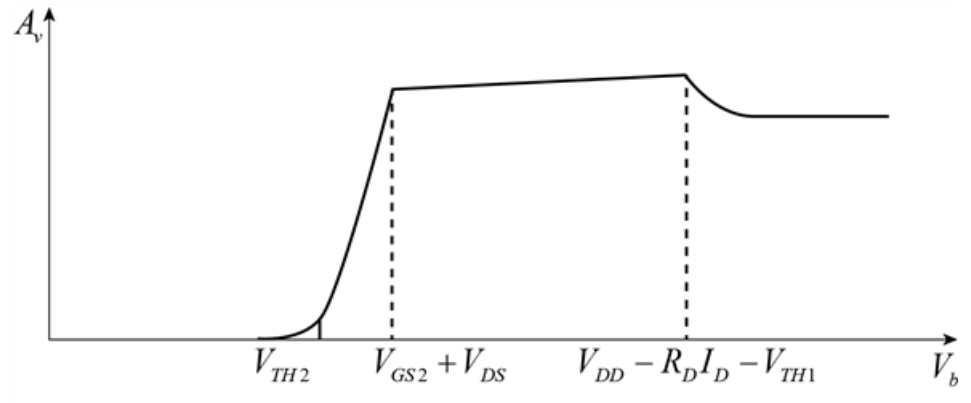
\includegraphics[width=1\linewidth]{3.28-1}
	\end{minipage}
	\caption*{图1} %最终文档中希望显示的图片标题
\end{figure}

$V_X \approx V_b-V_{TH2}$,当$V_b<V_{TH2}$时$V_{DS1}=V_X<0$,根据线性区公式$M_1$无电流。

当$V_b$稍大于$V_{TH2}$时$M_1$有电流,输出电压降低,$V_{GS2}$随着漏电流增大而增大并造成$V_X$降低。结果$M_1$在线性区$M_2$在饱和区。$V_b$增大导致$V_{DS1}$增大,$M_1$的输出电阻类似的增大\textcolor{blue}{($r_o \approx \frac{1+ \lambda V_{DS}}{\lambda I_D}$见教材P30的式2.47)},共源共栅级的电压增益增大。

$M_1,M_2$都在饱和区后,随着$V_b$增大$M_1$跨导增大,增益略有增加。

当$V_{out}$和$V_X$几乎相等时$M_2$在线性区。因此总输出阻抗减小,从而小信号电压增益相似地减小。






